\PassOptionsToPackage{unicode=true}{hyperref} % options for packages loaded elsewhere
\PassOptionsToPackage{hyphens}{url}
%
\documentclass[10pt,xcolor=table,color={dvipsnames,usenames},ignorenonframetext,usepdftitle=false,french]{beamer}
\setbeamertemplate{caption}[numbered]
\setbeamertemplate{caption label separator}{: }
\setbeamercolor{caption name}{fg=normal text.fg}
\beamertemplatenavigationsymbolsempty
\usepackage{caption}
\captionsetup{skip=0pt,belowskip=0pt}
%\setlength\abovecaptionskip{-15pt}
\usepackage{lmodern}
\usepackage{amssymb,amsmath,mathtools,multirow}
\usepackage{float,hhline}
\usepackage{tikz}
\usepackage[tikz]{bclogo}
\usepackage{mathtools}
\usepackage{ifxetex,ifluatex}
\usepackage{fixltx2e} % provides \textsubscript
\ifnum 0\ifxetex 1\fi\ifluatex 1\fi=0 % if pdftex
  \usepackage[T1]{fontenc}
  \usepackage[utf8]{inputenc}
  \usepackage{textcomp} % provides euro and other symbols
\else % if luatex or xelatex
  \usepackage{unicode-math}
  \defaultfontfeatures{Ligatures=TeX,Scale=MatchLowercase}
\fi
\usetheme[coding=utf8,language=french,
,titlepagelogo=img/LOGO-ENSAE.png
]{TorinoTh}
% use upquote if available, for straight quotes in verbatim environments
\IfFileExists{upquote.sty}{\usepackage{upquote}}{}
% use microtype if available
\IfFileExists{microtype.sty}{%
\usepackage[]{microtype}
\UseMicrotypeSet[protrusion]{basicmath} % disable protrusion for tt fonts
}{}
\IfFileExists{parskip.sty}{%
\usepackage{parskip}
}{% else
\setlength{\parindent}{0pt}
\setlength{\parskip}{6pt plus 2pt minus 1pt}
}
\usepackage{hyperref}
\hypersetup{
            pdftitle={Word-Embedding et sentiments des ménages avec Twitter},
            pdfauthor={Kim Antunez, Romain Lesauvage et Alain Quartier-la-Tente},
            pdfborder={0 0 0},
            breaklinks=true}
\urlstyle{same}  % don't use monospace font for urls
\newif\ifbibliography
% Prevent slide breaks in the middle of a paragraph:
\widowpenalties 1 10000
\raggedbottom
\AtBeginPart{
  \let\insertpartnumber\relax
  \let\partname\relax
  \frame{\partpage}
}
\AtBeginSection{
  \ifbibliography
  \else
    \begin{frame}{Sommaire}
    \tableofcontents[currentsection, hideothersubsections]
    \end{frame}
  \fi
}
\setlength{\emergencystretch}{3em}  % prevent overfull lines
\providecommand{\tightlist}{%
  %\setlength{\itemsep}{0pt}
  \setlength{\parskip}{0pt}
  }
\setcounter{secnumdepth}{0}

% set default figure placement to htbp
\makeatletter
\def\fps@figure{htbp}
\makeatother

\usepackage{wrapfig}
\usepackage{booktabs}
\usepackage{longtable}
\usepackage{array}
\usepackage{multirow}
\usepackage{wrapfig}
\usepackage{float}
\usepackage{colortbl}
\usepackage{pdflscape}
\usepackage{tabu}
\usepackage{threeparttable}
\usepackage{threeparttablex}
\usepackage[normalem]{ulem}
\usepackage{makecell}
\usepackage{animate}
\usepackage{fontawesome5}
\usepackage{caption}
\usepackage{graphicx}
\usepackage{tikz}
\usetikzlibrary{fit,arrows.meta}
\usepackage{pifont}
\usepackage{enumitem}
\usepackage{dsfont}
\setlist[itemize,1]{label = --}
\setlist[itemize,2]{label = $\circ$}
\setlist[enumerate,1]{label={\arabic*}}
\usepackage{lmodern}
\usepackage{cancel}
\usepackage{array}

\title{\emph{Word-Embedding} et sentiments des ménages avec Twitter}
\ateneo{Projet de statistique appliquée, Ensae}
\author{Kim Antunez, Romain Lesauvage et Alain Quartier-la-Tente}
\date{}


\setrellabel{}

\setcandidatelabel{}

\rel{}
\division{11/06/2020}

\departement{Ensae --- 2019-2020}
\makeatletter
\let\@@magyar@captionfix\relax
\makeatother

\DeclareMathOperator{\Cov}{Cov}
\newcommand{\E}[1]{\mathbb{E}\left[ #1 \right]}
\newcommand{\V}[1]{\mathbb{V}\left[ #1 \right]}
\newcommand{\cov}[2]{\Cov\left( #1\,,\,#2 \right)}

\begin{document}
\begin{frame}[plain,noframenumbering]
\titlepage
\end{frame}

\hypertarget{introduction}{%
\section{Introduction}\label{introduction}}

\begin{frame}{Introduction}
\protect\hypertarget{introduction-1}{}

\resizebox{\textwidth}{!}{\tikzstyle{myboxnorm} = [very thick,
    rectangle, rounded corners, inner sep=2pt, inner ysep=3pt, right,
    align=center]
\tikzstyle{myboxw2v} = [draw=red!50, fill=orange!10, myboxnorm]
\tikzstyle{myboxmod} = [draw=blue!60!green, fill=blue!5, myboxnorm]
\tikzstyle{myboxcomp} = [draw=green!50!black, fill=green!5, myboxnorm]

\tikzstyle{titlenorm} = [fill=white, very thick,
    rectangle, inner sep=2pt, inner ysep=2pt,font=\bfseries,
    text width=4.2cm, above=-0.3cm, align=center,
    minimum height=1.15cm]
\tikzstyle{titlew2v} = [draw=red!50, text = red!50,titlenorm]
\tikzstyle{titlemod} = [draw=blue!60!green,text=blue!60!green,titlenorm]
\tikzstyle{titlecomp} = [draw=green!50!black,text=green!50!black, titlenorm]    

\tikzstyle{fleche} = [->,rounded corners,line width=1pt]

\begin{tikzpicture}
\usetikzlibrary{fit}
\usetikzlibrary{arrows.meta}
%Il faut d'abord faire les boites
% w2vec
\node[fit={(2.5,1.5) (-3.,-3.5)}, myboxw2v,semitransparent] (w2vrect) {};
\node[fit={(2.7,1.5) (8.2,-5.5)}, myboxmod,semitransparent] (rectmod) {};
\node[fit={(13.9,1.5) (8.4,-5.5) }, myboxcomp,semitransparent] (rectcomp) {};

\node at (0,0) [myboxw2v] (tweets) {Tweets};
\node at (2.4,0) [myboxw2v] (we) {\textit{word-embedding}};
% sentiment
\node at (0,-4.5) [myboxnorm,text width=2.5cm, draw = black] (bddsent) {Échantillon de tweets annotés
};

% analyse de sentimentsentiment
\node at (7,0) [myboxmod] (logit) {Modèle logit};
\node at (7,-4.5) [myboxmod,text width=2.22cm] (baseline) {Modèle lexical};

% analyse de sentimentsentiment
\node at (12,0) [myboxcomp,text width=3.8cm] (indsent) {Indices mensuels de \\sentiment des tweets};

\node at (12,-4.5) [myboxcomp,text width=3.8cm] (camme) {Indicateur synthétique \\de confiance des

ménages (Insee)};

%Fleches
\draw[fleche] (tweets.east) --(we.west) node[below = 0.2cm,pos=1]{
\begin{minipage}{5cm} \footnotesize
  \begin{itemize}[label=\scalebox{.6}{\ding{110}}] 
  \item tokénisation
  \item choix hyperparamètres
  \item évaluation : 
  \begin{itemize}[label=\scalebox{.6}{\ding{117}}]
    \item similarité cosinus
    \item réduction de dimension (ACP/TSNE)
    \item jugement humain
  \end{itemize}
  \end{itemize} 
\end{minipage} 
};
\draw[fleche] (bddsent.east)--(baseline.west) 
  node[pos=0.36,text width=3cm]{
    \footnotesize bases  
    
    test/entraînement}
  node[pos=0.96, below = 0.05cm,text width=2.5cm]{
    \footnotesize sentiment 
    
    moyen d'un mot};
\draw[fleche] (bddsent.east)--++(2,0)--++(0,0.8)-|(logit.south);
\draw[fleche] (we.east)--(logit.west)node[pos=0.89,text width=2.5cm]{\footnotesize \emph{sentence}
  
  \emph{embedding}};
\draw[fleche] (logit.east)--
  (indsent.west)node[pos=0.62,text width=2.5cm]{\footnotesize moyennes
  
  mensuelles};
\draw[fleche] (baseline.east)-|(9.6,0)--(indsent.west);
\draw[fleche,<->] (indsent.south)--(camme.north) 
  node[pos=.5,text width=2.5cm, right=0.2cm]{\footnotesize distance entre
  
  indicateurs}
  node[pos=.5,text width=1.7cm, left]{\footnotesize prévision /
  
  causalité};

\node[titlew2v] at (w2vrect.north) { word2vec \\
(skip-gram)};
\node[titlemod] at (rectmod.north) { Analyse de \\
sentiment d'un tweet};
\node[titlecomp] at (rectcomp.north) { Comparaison \\
d'indices mensuels};
\end{tikzpicture}}

\end{frame}

\hypertarget{word2vec}{%
\section{\texorpdfstring{\emph{word2vec}}{word2vec}}\label{word2vec}}

\hypertarget{uxe9valuation-du-moduxe8le}{%
\section{Évaluation du modèle}\label{uxe9valuation-du-moduxe8le}}

\hypertarget{uxe9valuation-sur-un-corpus-fictif}{%
\subsection{Évaluation sur un corpus
fictif}\label{uxe9valuation-sur-un-corpus-fictif}}

\begin{frame}{Comment évaluer le modèle ?}
\protect\hypertarget{comment-uxe9valuer-le-moduxe8le}{}

\textbf{Problème} : utilisation généralisée des \emph{word-embeddings}
mais peu de travaux théoriques expliquent ce qui est capturé, comment
évaluer le modèle ?

\faArrowCircleRight{} Utiliser un corpus fictif.

Les vecteurs-mots sont de grande dimension : comment juger de leur
proximité ?

\begin{itemize}
\item
  Distance entre mots mesurée par distance euclidienne ou
  \textbf{similarité cosinus}.
\item
  \textbf{ACP} : réduire la dimension et analyser les proximités.
\item
  \textbf{t-SNE} : algorithme stochastique qui favorise l'apparition de
  clusters.
\item
  \textbf{Jugement humain} : corrélations entre mots faites par l'homme,
  utilisées comme références.
\end{itemize}

\end{frame}

\begin{frame}{Évaluation sur un corpus fictif}
\protect\hypertarget{uxe9valuation-sur-un-corpus-fictif-1}{}

\textbf{Idée} : construire un corpus fictif pour lesquels on connaît le
résultat attendu en contrôlant les contextes.

\textbf{En pratique} :

\begin{itemize}
\item On génère 10 groupes de mots composés d'un couple de référence et de 10 autres mots contexte.
\item On construit 10 000 phrases en tirant au hasard :
\begin{itemize}
\item 1 des groupes de mots ;
\item 1 des 2 mots \og références \fg{} du groupe ;
\item 5 mots contextes ;
\item 3 mots bruits parmi une liste de 100 mots.
\end{itemize}
\item On mélange les 9 mots de chaque phrase.
\end{itemize}

\end{frame}

\begin{frame}{Résultats de l'évaluation}
\protect\hypertarget{ruxe9sultats-de-luxe9valuation}{}

\begin{table}[!h]
\begin{center}
\begin{tabular}{|c|>{\centering\arraybackslash}p{3cm}|}
    \hline
    mot & similarité cosinus avec \og grand \fg{} \tabularnewline
    \hline
    longueur & 0,982   \tabularnewline
    petit & 0,981   \tabularnewline
    s & 0,979   \tabularnewline
    $\vdots$ & $\vdots$    \tabularnewline
    susiens & $- 0,735$ \tabularnewline
    allates & $-0,784$ \tabularnewline
    %produit & 0,100   \tabularnewline
    %voiture & 0,097   \tabularnewline
    \hline
 \end{tabular}
\begin{tabular}{|c|>{\centering\arraybackslash}p{3cm}|}
    \hline
    mot & similarité cosinus avec \og petit \fg{} \tabularnewline
    \hline
    taille & 0,987   \tabularnewline
    longueur & 0,983   \tabularnewline
    grand & 0,981   \tabularnewline
    $\vdots$ & $\vdots$    \tabularnewline
    alesiez & $- 0,745$ \tabularnewline
    allates & $-0,810$ \tabularnewline
    %citrine & 0,129   \tabularnewline
    %voiture & 0,121   \tabularnewline
    \hline
 \end{tabular}
\end{center}
\footnotesize
\emph{Note : Paramètres utilisés : ep = 50 / lr = 0,01 / w = 5 / dim = 10.}
\end{table}

On obtient de très bon résultats conformes à ce qui était attendu :
l'implémentation du modèle semble validée.

\end{frame}

\hypertarget{choix-des-meilleurs-hyperparamuxe8tres-pour-le-moduxe8le}{%
\subsection{Choix des meilleurs hyperparamètres pour le
modèle}\label{choix-des-meilleurs-hyperparamuxe8tres-pour-le-moduxe8le}}

\begin{frame}{Choix des meilleurs hyperparamètres pour le modèle}
\protect\hypertarget{choix-des-meilleurs-hyperparamuxe8tres-pour-le-moduxe8le-1}{}

\begin{itemize}
\item
  \textit{word2vec} se base sur différents choix d'hyperparamètres :
  taille de la fenêtre (\textit{w}), nombre d'epochs (\textit{ep}), taux
  d'apprentissage (\textit{lr}), dimension des \textit{word-embeddings}
  (\textit{dim}).
\item
  Meilleurs valeurs des hyperparamètres déterminées de manière
  empirique.
\item
  Mesure des résultats : utilisation d'un corpus de jugement humain et
  étude des corrélations de Spearman entre ce corpus et notre modèle.
\item
  Problème de temps de compilation de notre algorithme : il faut
  relancer le modèle à chaque fois.
\item
  Utilisation complémentaire de \textbf{Gensim} puis résultats validés
  avec notre implémentation.
\end{itemize}

\end{frame}

\begin{frame}{Nombre d'epochs, taille de fenêtre et taux
d'apprentissage}
\protect\hypertarget{nombre-depochs-taille-de-fenuxeatre-et-taux-dapprentissage}{}

\begin{figure}[htp]
\begin{center}
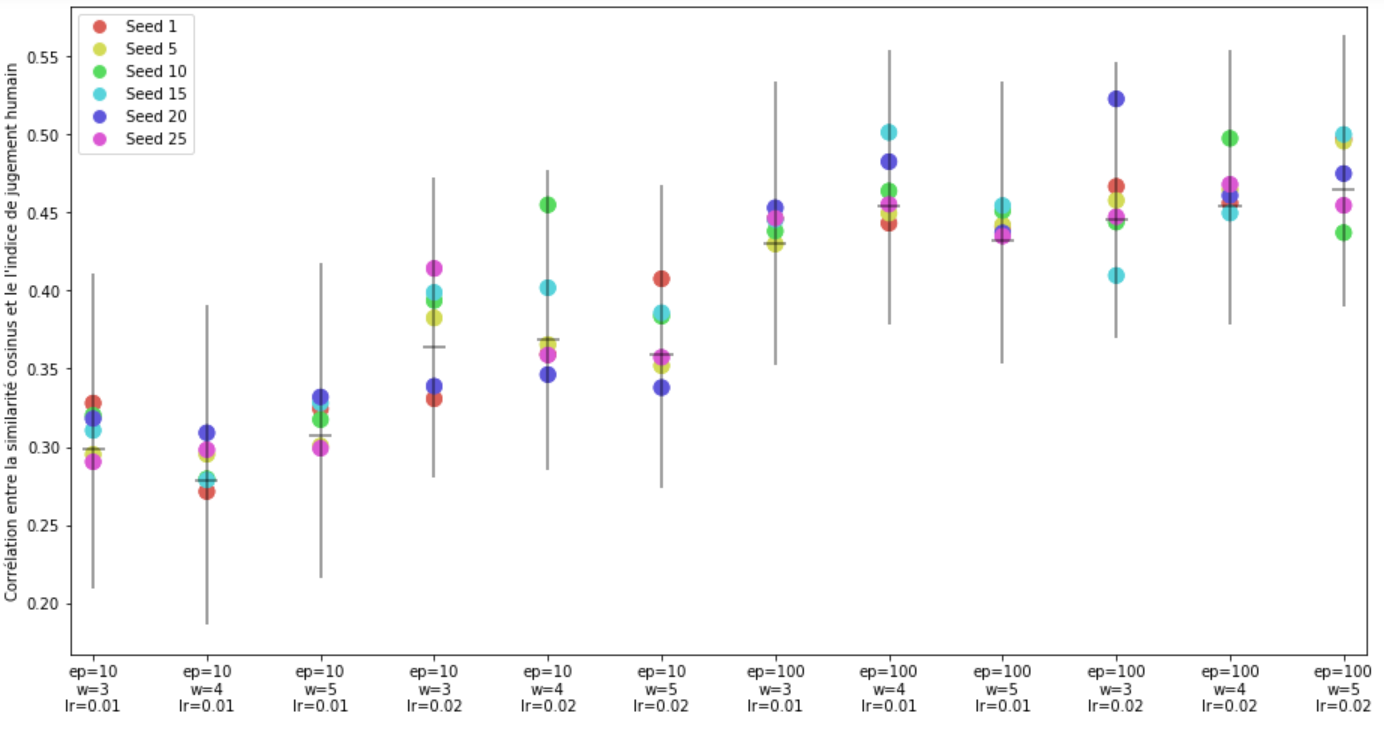
\includegraphics[width=1\textwidth]{img/test_parametres.png}
\end{center}
\vspace{-0.3cm}
\footnotesize
\emph{Note : Paramètre utilisé : dim = 50}
\end{figure}

\end{frame}

\begin{frame}{Valeurs des hyperparamètres retenus}
\protect\hypertarget{valeurs-des-hyperparamuxe8tres-retenus}{}

\begin{itemize}

\item \textbf{Nombre d'epochs} : augmentation du nombre d'epochs améliore les résultats

\faArrowCircleRight{} \textbf{ep = 100}.

\item \textbf{Taille de fenêtre} : capture différentes informations selon valeur

\faArrowCircleRight{} \textbf{w = 4}.

\item \textbf{Taux d'apprentissage} : 0,02 donne de meilleurs résultats

\faArrowCircleRight{} \textbf{lr = 0,02}.
\end{itemize}

Pour la dimension des vecteurs-mots, on observe une amélioration des
résultats en augmentant la dimension jusqu'à atteindre 300. En réalité,
peu de différences ici entre 100 et 300 \faArrowCircleRight{}
\textbf{dim = 100} par soucis de temps de compilation.

\end{frame}

\hypertarget{uxe9valuation-sur-le-corpus-de-tweets}{%
\subsection{Évaluation sur le corpus de
tweets}\label{uxe9valuation-sur-le-corpus-de-tweets}}

\begin{frame}{Évaluation sur le corpus de tweets (1/2)}
\protect\hypertarget{uxe9valuation-sur-le-corpus-de-tweets-12}{}

\begin{figure}
\begin{minipage}{.4\textwidth}


« Notre » modèle

\medskip

\footnotesize
\textbf{ Spearman : } 0,57 (p-v : 4,1 \%)
\normalsize

\medskip

\faArrowCircleRight{} \textbf{bons} résultats


\end{minipage}%
\begin{minipage}{.6\textwidth}
\tiny

\begin{table}[!h]
\begin{center}
\begin{tabular}{|c|c|c|c|}
    \hline
\textbf{bonjour} & \textbf{femme} & \textbf{1} & \textbf{samedi} \tabularnewline
\emph{(669)} & \emph{(264)} & \emph{(765)} & \emph{(203)} \tabularnewline
       \hline

\includegraphics[height=2mm]{img/emojis/1.png} (0,59) & quelle (0,49) & 5 (0,55) & soir (0,57) \tabularnewline

\includegraphics[height=2mm]{img/emojis/2.png} (0,59) & cette (0,46) & mois (0,51) & vivement (0,51) \tabularnewline
merci (0,54) & une (0,44) & 10 (0,49) & demain (0,50) \tabularnewline
nuit (0,48) & vie (0,44) & 2 (0,48) & end (0,48) \tabularnewline
bisous (0,47) & grippe (0,44) & top (0,48) & weekend (0,47) \tabularnewline
bonne (0,47) & belle (0,43) & depuis (0,47) & matin (0,45) \tabularnewline

\includegraphics[height=2mm]{img/emojis/3.png} (0,46) & ma (0,43) & saison (0,46) & jeudi (0,45) \tabularnewline
vous (0,46) & magnifique (0,43) & ans (0,44) & prochain (0,43) \tabularnewline
plaisir (0,44) & nouvelle (0,43) & jours (0,43) & week (0,43) \tabularnewline
allez (0,43) & vidéo (0,39) & 3 (0,43) & 
\includegraphics[height=2mm]{img/emojis/4.png} (0,42) \tabularnewline
    \hline
 \end{tabular}
\captionsetup{margin=0cm,format=hang,justification=justified}

\end{center}
\emph{ep = 80 / w = 4 / lr = 0,02 / dim = 100 / base : 100 000 tweets}

\end{table}
\normalsize


\end{minipage}
\end{figure}

\pause

\begin{figure}
\begin{minipage}{.4\textwidth}

Modèle \texttt{Gensim}

\medskip

\footnotesize
\textbf{ Spearman : } 0,50 (p-v : 0,0 \%)
\normalsize

\medskip

\faArrowCircleRight{} \textbf{très bons} résultats

\end{minipage}%
\begin{minipage}{.6\textwidth}
\tiny

\begin{table}[h]
\begin{center}
\begin{tabular}{|c|c|c|c|}
    \hline
\textbf{bonjour} & \textbf{femme} & \textbf{1} & \textbf{samedi} \tabularnewline
\emph{(17 043)} & \emph{(6 177)} & \emph{(21 055)} & \emph{(4 917)} \tabularnewline
       \hline
bonsoir (0,85) & fille (0,86) & 2 (0,65) & vendredi (0,88) \tabularnewline
bjr (0,75) & copine (0,74) & 3 (0,64) & jeudi (0,86) \tabularnewline
hello (0,71) & meuf (0,71) & 6 (0,63) & lundi (0,83) \tabularnewline
salut (0,66) & demoiselle (0,66) & 4 (0,62) & mercredi (0,83) \tabularnewline
coucou (0,55) & nana (0,66) & 7 (0,60) & dimanche (0,83) \tabularnewline
transmets (0,49) & nièce (0,66) & 5 (0,58) & mardi (0,76) \tabularnewline
désagrément (0,48) & sœur (0,65) & 9 (0,58) & demain (0,72) \tabularnewline
avezvous (0,48) & barbe (0,65) & 8 (0,56) & barathon (0,56) \tabularnewline
bettembourg (0,48) & maman (0,64) & 1e (0,55) & 22h45 (0,55) \tabularnewline
hey (0,47) & princesse (0,64) & 34 (0,53) & 20h (0,54) \tabularnewline
    \hline
 \end{tabular}
\captionsetup{margin=0cm,format=hang,justification=justified}
\end{center}
\emph{ep = 100 / w = 4 / lr = 0,02 / dim = 100 / base : ensemble des tweets}

\medskip

\footnotesize{10 plus proches voisins par similarité cosinus}
\end{table}

\normalsize

\end{minipage}
\end{figure}

\end{frame}

\begin{frame}{Évaluation sur le corpus de tweets (2/2)}
\protect\hypertarget{uxe9valuation-sur-le-corpus-de-tweets-22}{}

\begin{figure}
\begin{minipage}{.5\textwidth}

\begin{center}
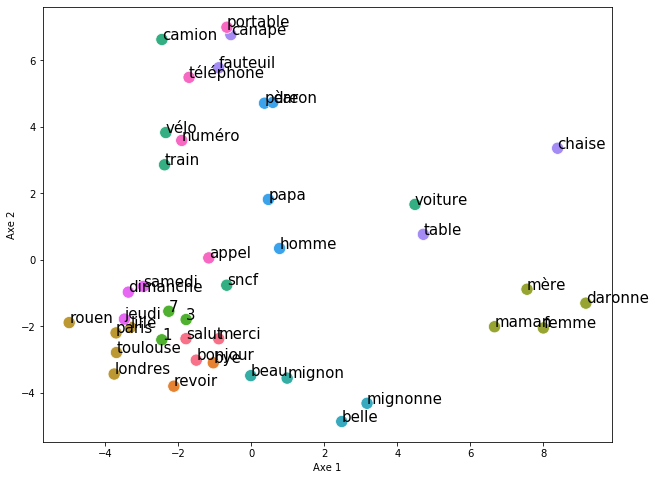
\includegraphics[width=0.95\textwidth]{img/acp_gensim.png}
\end{center}
\emph{ACP sur un corpus réduit de mots.}


\end{minipage}%
\begin{minipage}{.5\textwidth}

  \centering
  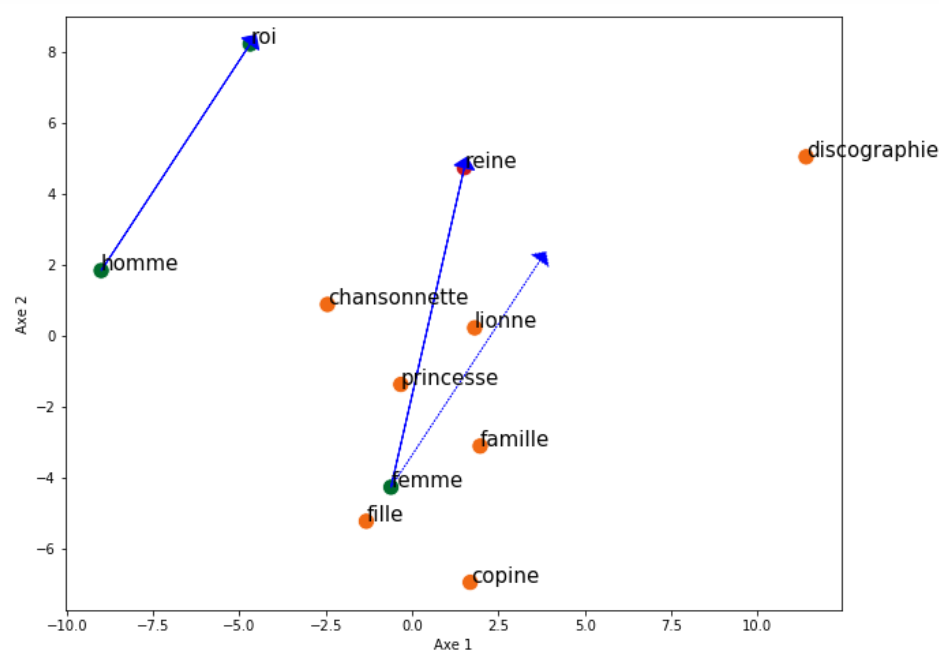
\includegraphics[width=\linewidth]{img/acp_reine.png}
  \emph{$\protect\overrightarrow{Roi} - \protect\overrightarrow{Homme} + \protect\overrightarrow{Femme} = $ ?}

\end{minipage}

\end{figure}

\medskip

\faArrowCircleRight{} Réduction de dimension des vecteurs-mots et
(parfois) opérations sur les mots \textbf{convaincants}

\end{frame}

\hypertarget{indice-de-sentiments}{%
\section{Indice de sentiments}\label{indice-de-sentiments}}

\hypertarget{pruxe9dire-le-sentiment-dun-tweet}{%
\subsection{Prédire le sentiment d'un
tweet}\label{pruxe9dire-le-sentiment-dun-tweet}}

\begin{frame}{Prédire le sentiment d'un tweet}
\protect\hypertarget{pruxe9dire-le-sentiment-dun-tweet-1}{}

\textbf{Idée} : associer à chaque tweet un sentiment qui vaut 1 s'il est
positif et 0 s'il est négatif.

Pour cela, nous avons à notre disposition une base de tweets annotés sur
les transports urbains, contenant 23 000 tweets, séparée en une base de
\emph{train} (16 000 tweets) et de \emph{test} (7 000 tweets).

2 approches ici :

\begin{itemize}
\item Modèle lexical : utiliser l'information des tweets labelisés pour construire un sentiment moyen par mot.
\item Modèle \textit{logit} : utiliser nos \textit{word-embeddings} comme prédicteurs d'une régression logistique.
\end{itemize}

\end{frame}

\begin{frame}{Modèle lexical : sentiment moyen des mots}
\protect\hypertarget{moduxe8le-lexical-sentiment-moyen-des-mots}{}

Le sentiment prédit d'un tweet \(t\) composé de \(n\) mots sera :
\[S_{1,\gamma}(t) = \mathds{1}\left\{ \frac{1}{n} \sum \limits_{i=1}^n \alpha_i \geq \gamma\right\}  \qquad \in \{ 0,1 \}\]

\begin{itemize}
\item $\gamma \in [-1,1]$ un seuil fixé ;
\item $\alpha_i = \frac{nb_+(i) - nb_-(i)}{nb_+(i) + nb_-(i)} \in [-1,1]$  sentiment moyen du mot $i$ calculé à partir du nombre de tweets positifs ($nb_+(i)$) et négatifs ($nb_-(i)$) dans lesquels il apparaît. 
\end{itemize}

On détermine le \(\gamma\) optimal en regardant l'\emph{accuracy} sur la
base de train : on trouve \(\gamma^*\) = -0.14 pour une \emph{accuracy}
(sur la base de test) de \textbf{89.1\%}.

\end{frame}

\begin{frame}{Modèle logit : prédiction grâce aux
\emph{word-embeddings}}
\protect\hypertarget{moduxe8le-logit-pruxe9diction-gruxe2ce-aux-word-embeddings}{}

\[
Y_i = 1\left\{ \sum_{i = 1}^n \beta_i X_{i,j} + \varepsilon_i \geq 0 \right\} 
\] \[
\mathbb{P}(Y_i = 1 | X_{i}) = F_{\varepsilon}\left(\sum_{i = 1}^n \beta_i X_{i,j}\right)
\]

\begin{itemize}
\item $Y_i$ le sentiment du tweet $i$ ;
\item $X_{i,1}, \dots, X_{i,n}$ les coordonnées de la \emph{sentence-embedding} du tweet $i$ ;
\item $\varepsilon_i$ le résidu de notre modèle, de fonction de répartition $F_{\varepsilon}$ qui vaudra $F_{\varepsilon}(x) = \frac{1}{1 + e^{-x}}$ dans le cas d'un modèle logit et $F_{\varepsilon}(x) = \Phi(x)$ (fonction de répartition d'une loi $\mathcal{N}(0, 1)$) dans le cas d'un modèle probit. 
\end{itemize}

\end{frame}

\begin{frame}{Spécifications du modèle logit}
\protect\hypertarget{spuxe9cifications-du-moduxe8le-logit}{}

Plusieurs problèmes à traiter :

\begin{itemize}
\item
  Doit-on inclure les \emph{stop-words} ? \faArrowCircleRight{} On
  décide de les garder.
\item
  Comment traiter les mots inconnus ? \faArrowCircleRight{} On décide de
  leur affecter le vecteur du mot \emph{lowfrequency}.
\item
  Modèle probit ou logit ? \faArrowCircleRight{} On retient le modèle
  logit.
\end{itemize}

Le sentiment du tweet \(t\) est :

\[S_{2,\gamma}(t) = 1\left\{   \mathbb{P}(Y_i = 1 | X_{i}) \ge \gamma\right\} \qquad \in \{0,1\}\]

On détermine le \(\gamma\) optimal en regardant l'\emph{accuracy} sur la
base de train : on trouve \(\gamma^*\) = 0.5 pour une \emph{accuracy}
(sur la base de test) de \textbf{69.8\%}.

\end{frame}

\begin{frame}{Limites des modèles utilisés}
\protect\hypertarget{limites-des-moduxe8les-utilisuxe9s}{}

La bonne performance du modèle lexical par rapport au modèle logit peut
s'expliquer par plusieurs facteurs.

\begin{enumerate}
\tightlist
\item
  Les mots inconnus diffèrent selon les modèles. Modèle lexical : 1,4 \%
  des mots sont inconnus (13,2 \% du vocabulaire) Modèle logit : 4,6 \%
  des mots sont inconnus (36,2 \% du vocabulaire)
\end{enumerate}

\pause

\begin{enumerate}
\setcounter{enumi}{1}
\tightlist
\item
  Le processus d'annotation utilisé pour les tweets sur les transports
  urbains.
\end{enumerate}

\pause

\begin{enumerate}
\setcounter{enumi}{2}
\tightlist
\item
  Le \emph{domain shift} \pause Utilisation d'une nouvelle base de test
  indépendante pour essayer de neutraliser ces effets : \textbf{modèle
  logit meilleur que le modèle lexical} (61,9~\% contre 55,9~\%).
\end{enumerate}

\end{frame}

\begin{frame}{Merci pour votre attention}
\protect\hypertarget{merci-pour-votre-attention}{}

\href{https://github.com/ARKEnsae/TweetEmbedding}{\faGithub{} ARKEnsae/TweetEmbedding}

\href{https://arkensae.github.io//TweetEmbedding/Redaction/Rapport_Final/Rapport.pdf}{\faEdit{} Rapport du projet}

\begin{center}

\includegraphics[width = 2.5cm]{img/LOGO-ENSAE.png}
\end{center}

\end{frame}

\end{document}
